\section{Design}
\label{design}
BLS-CoSi is designed for sparse communication pattern over the network. The nodes are arranged in a 3-level tree structure. The node at the root acts as the leader of the tree and the remaining non-leaf nodes act as the sub-leader of their corresponding subtree.

The BLS-CoSi protocol runs as follows:\\
1) The root initiates the protocol by multicasting the message to be signed to its children, who further multicast it down the tree.\\
2) Each leaf node, $n_i$ responds by returning the signature $\sigma_i$ signed by their own private key. The subleader aggregates the received signatures along with their own signature and sends it to the root. The root, similarly aggregates the received aggregated signatures and the own signature to generate a single collective-signature, that is sent to the client.

The single-round trip protocol eliminates the risk faced in the two-round CoSi where the nodes not participating in the first round might disappear in the second round. Therefore BLSCoSi is useful in highly unstable networks. BLS signatures can be aggregated incrementally thus allowing participants to generate fast responses on an asynchronous network.

Non-responsive nodes do not affect the availability of the protocol. If the subleader fails to respond within a specified time period, the subtree is reorganized with a new subleader is initiated. The unresponsive leaf nodes are simply not included during aggregation.
\begin{figure}[h]
	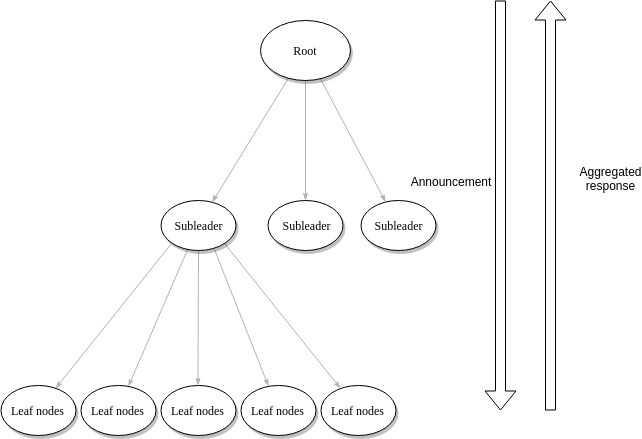
\includegraphics[width=10cm]{bls.png}
	\caption{Design of BLSCoSi}
	\label{fig}
\end{figure}
\clearpage